\chapter{Literature Review}
	\section{Image-to-Image Translation with Conditional Adversarial Networks\cite{isola2018imagetoimage}}
   Conditional Adversarial Networks are a promising approach for many image-to-image translation tasks, especially those involving highly structured graphical outputs. The paper introduces a conditional variant of GANs, which can be used for image-to-image translation tasks. The model learns a mapping from input images to output images. However due to lack of definite structure in manga and training data pairs this architecture fails to adapt for our purpose.
   \begin{figure}[htbp]
    \centering
    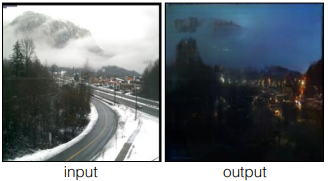
\includegraphics[width=0.4\textwidth]{img/model0.png}
    \caption{Realistic image colorization}
    \subcaption*{\textit{source: \textcolor{blue}{https://arxiv.org/pdf/1611.07004v1.pdf}}}
    \label{fig:Model-0}
  \end{figure}
    \section{Manga Colorization Using Reference Images\cite{qu2006manga}}
    Colourizing manga by tracing pattern continuity and intensity continuity.
	Intensity continuity to avoid colour bleeding. This is manual and proper edge detection is not possible with the pattern continuity method.
    \begin{figure}[htbp]
    \centering
    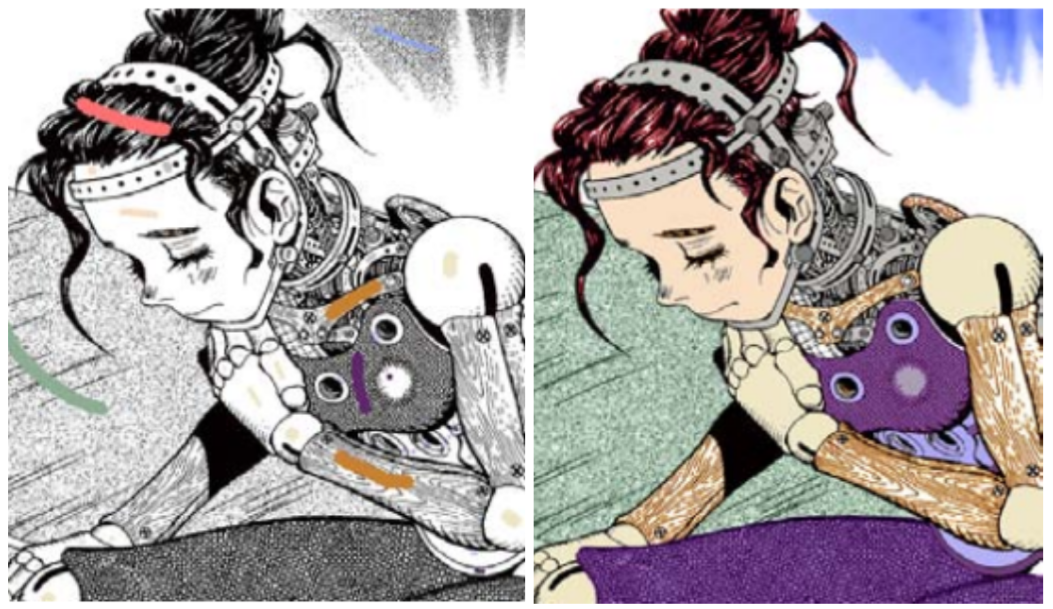
\includegraphics[width=0.4\textwidth]{img/model1.png}
    \caption{Colorization using pattern continuity}
    \subcaption*{\textit{source: \textcolor{blue}{https://www.youtube.com/watch?v=HpZUOq3O64s}}}
    \label{fig:Model-1}
  \end{figure}
    \newpage
    \section{cGAN-based Manga Colorization Using a Single Training Image\cite{hensman2017cganbased}}
    They used cGAN based approach for colorization along with segmentation of manga to produce high resolution and clean images.This method fails to generalise colorization for diverse characters and suffers heavily from colour monotonicity. 
    \begin{figure}[htbp]
        \centering
        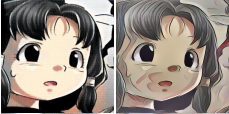
\includegraphics[width=0.6\textwidth]{img/model2.png}
        \caption{Colorization using single image reference}
        \subcaption*{\textit{source: \textcolor{blue}{https://arxiv.org/pdf/1706.06918.pdf}}}
        \label{fig:Model-2}
      \end{figure}

    \section{Style Transfer for Anime Sketches with Enhanced Residual U-net and Auxiliary Classifier GAN\cite{ACPR2017ZLM}}
    Style maps and colour hints must be provided by the user for this network to perform colorization. Also the pretrained VGG is used which performs best for classification, but not for paintings.
    \begin{figure}[htbp]
        \centering
        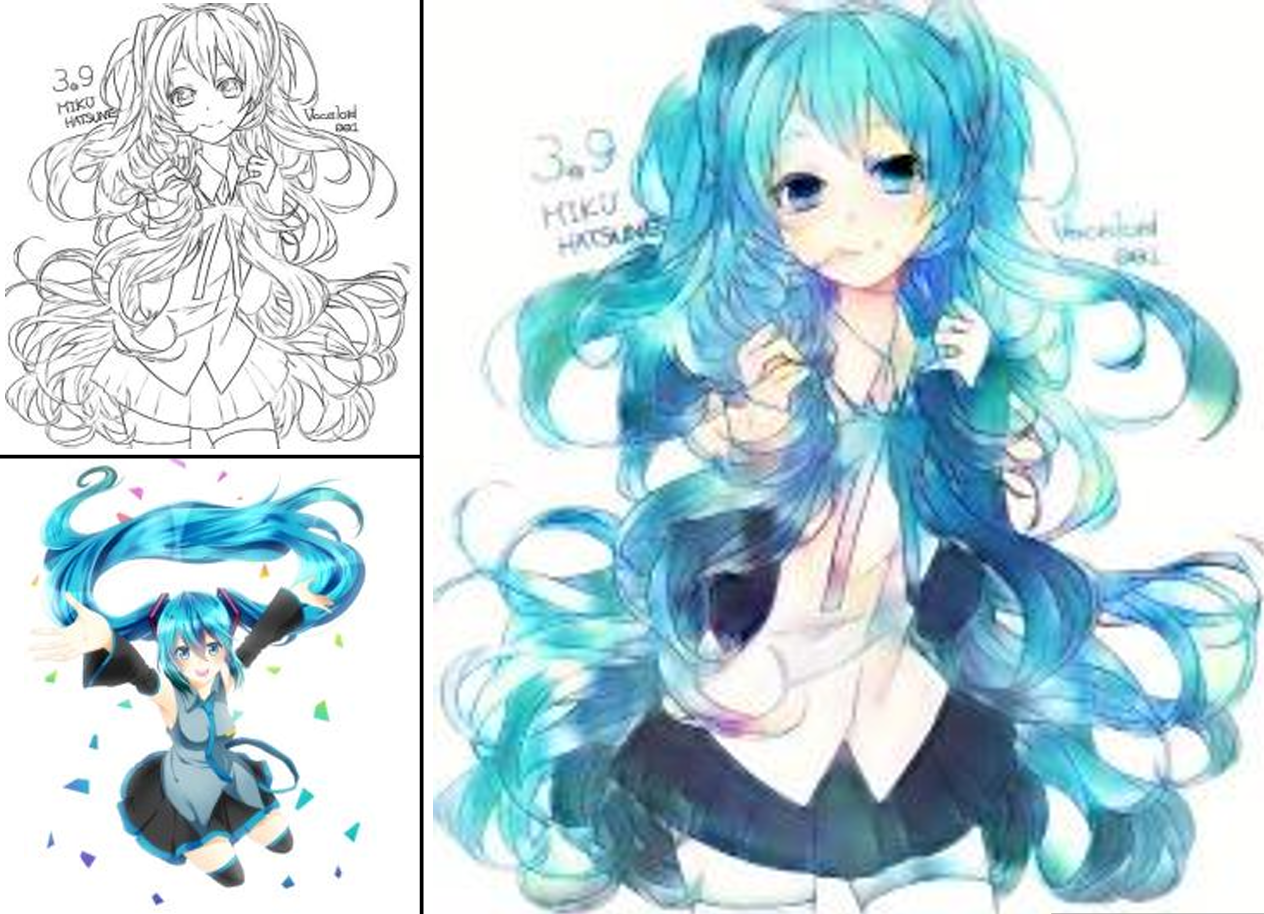
\includegraphics[width=0.6\textwidth]{img/model3.png}
        \caption{Colorization using style transfer method.}
        \subcaption*{\textit{source: \textcolor{blue}{https://arxiv.org/pdf/1706.03319.pdf}}}
        \label{fig:Model-3}
      \end{figure}
\newpage
    \section{inkn’hue: Enhancing Manga Colorization from Multiple Priors with Alignment Multi-Encoder VAE and StyleGAN\cite{jiramahapokee2023inkn}}
    Failed to fully automate the colorization process as a colour hints and partially coloured image was required as input for custom post processing.
    \begin{figure}[htbp]
        \centering
        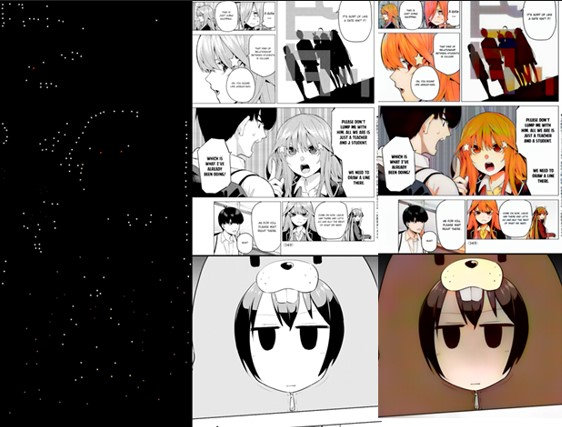
\includegraphics[height=0.4\textwidth]{img/model4.jpg}
        \caption{Semi-automatic colorization using multi-encoder VAE and StyleGAN}
        \subcaption*{\textit{source: \textcolor{blue}{https://arxiv.org/pdf/2311.01804.pdf}}}
        \label{fig:Model-4}
      \end{figure}
     \section{Semi-automatic Manga Colorization Using Conditional Adversarial Networks\cite{10.1007/978-3-030-72610-2_17}}
    If some object has several suitable colours, the neural network will produce a value
    close to the average of these colours that leads to degradation of the results, and monotone. 
    \begin{figure}[htbp]
        \centering
        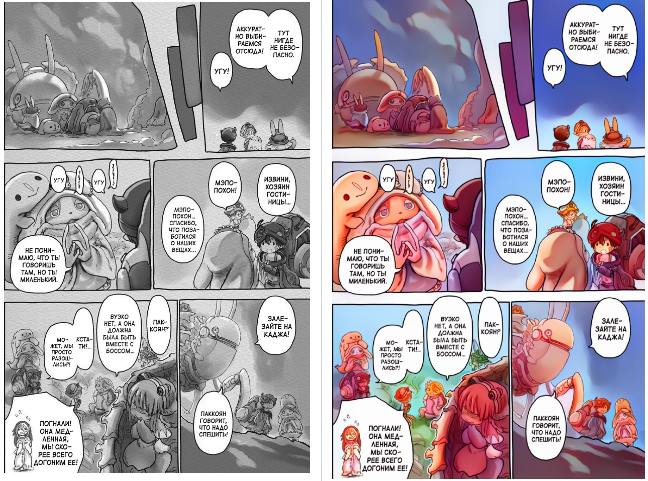
\includegraphics[width=0.5\textwidth]{img/model5.png}
        \caption{Semi-automatic colorization using cGAN}
        \subcaption*{\textit{source: \textcolor{blue}{https://github.com/qweasdd/manga-colorization-v2}}}
        \label{fig:Model-5}
      
      \end{figure}

\newpage
\section{Review Matrix}
\begin{table}[htp]
  \begin{tabular}{|c|p{4cm}|p{3cm}|p{4.5cm}|}
    \hline
    \textbf{S.N.} & \textbf{Title} & \textbf{Author(s)} & \textbf{Findings} \\ \hline
    
    1 & 
    Semi-automatic Manga Colorization Using Conditional Adversarial Networks \cite{10.1007/978-3-030-72610-2_17}  & 
    Maksim Golyadkin and Ilya Makarov &
    
    A cGAN-powntinuities, allowing users to personalize results with color hints and fine-tune for stylistic accuracy. \\ \hline

    2 & 
    Image-to-Image Translation with Conditional Adversarial Networks \cite{isola2018imagetoimage} & 
    Phillip Isola, Jun-Yan Zhu, Tinghui Zhou, and Alexei A. Efros & 
    This paper introduces cGAN for image-to-image translation, enabling the generation of realistic images by conditioning on input images from different domains. \\ \hline

    3 & 
    cGAN-based Manga Colorization Using a Single Training Image \cite{hensman2017cganbased} & 
    Kiyoharu Aizawa and Paulina Hensman &
    This method uses GANs to color entire manga pages, learning patterns and letting us personalize with hints and style tweaks. \\ \hline

    4 & Deep Extraction of x`Manga Structural Lines \cite{li-2017-deep} & Chengze Li, Xueting Liu, And Tien-Tsin Wong
    & It is a data-driven approach that uses CNN to identify structural lines in pattern-rich manga. \\ \hline

     5 & Style Transfer for Anime Sketches
    with Enhanced Residual U-net and Auxiliary Classifier GAN \cite{ACPR2017ZLM} &
    Lvmin Zhang, Yi Ji and Xin Lin & a method to apply the style of a painting to an anime sketch. \\ \hline

         \end{tabular}
\end{table}

\newpage

\begin{table}[htbp]
\centering
  \begin{tabular}{|c|p{4cm}|p{3cm}|p{4.5cm}|}
    \hline  
 
    6 & 
    Comicolorization: Semi-Automatic Manga Colorization \cite{furusawa2017comicolorization} & 
    Chie Furusawa, Kazuyuki Hiroshiba, Keisuke Ogaki and Yuri Odagiri & 
    This paper semi-automatically colorizes monochrome manga images using reference images, maintaining consistent colors for characters across panels, and allows for user revisions. 
    \\ \hline
  

    7 & Deep Residual Learning for Image Recognition \cite{he2015deep} & Kaiming He, Xiangyu Zhang, Shaoqing Ren, and Jian Sun & 
     This approach to convolution solves gradient vanishing problem allowing us to train very deep networks. 
     \\ \hline

    8 & U-Net: Convolutional Networks for Biomedical Image Segmentation \cite{ronneberger2015unet} & Olaf Ronneberger, Philipp Fischer, and Thomas Brox &
     Encoder and decoder architecture of U-net can be used for obtaining high resolution output and also enables 
     better image segmentation.
     \\ \hline

    9 & A Style-aware Discriminator for Controllable Image Translation \cite{kim2022styleaware} & Kunhee Kim, Sanghun Park, Eunyeong Jeon, Taehun Kim, and Daijin Kim &  
    The paper proposes a style-aware discriminator that acts as a critic and a style encoder to provide conditions which learns a controllable style space using prototype-based self-supervised learning and guides the generator.\cite{kim2022styleaware}
    \\ \hline

    10 & Wasserstein GAN \cite{arjovsky2017wasserstein} & Martin Arjovsky, Soumith Chintala, and Léon Bottou & This paper aims to solve mode collapse and hyperparameter sensitivity present in GANs using Wasserstein distance. 
    \\ \hline

    11 & Unpaired Image-to-Image Translation using Cycle-Consistent Adversarial Networks
    \cite{zhu2020unpaired} &
    Jun-Yan Zhu, Taesung Park, Phillip Isola, Alexei A. Efros & Style transfer between two sets of unpaired image dataset is possible. 
    \\ \hline
    
 \end {tabular}
  \caption{ Review Matrix with Research Papers, Authors, and Findings.}
  \label{tab:literature}
\end{table}
